\subsection{Processes}

A process is a program in execution.
A program is a passive entity stored on the disk, whereas a process is an active entity.
A program becomes a process when its executable file is loaded into memory.

A program may be started through a GUI or CLI\@.
One program may consist of several processes.
For example, there may be one process for each user or instance.

Processes are represented by three main components.
\begin{itemize}
  \item Executable program code (also known as the `text segment')
  \item Data related to the program
  \item Execution context
  \begin{itemize}
    \item process ID, group ID, user ID
    \item stack pointer, program counter, CPU registers
    \item file descriptors, locks, network sockets
  \end{itemize}
\end{itemize}
The execution context is essential for process switching.

A process can be an execution environment for other code.
For example, the JVM executes as a process that interprets loaded Java code and performs instructions on behalf of it.

\subsection{Process Structure}

A process is more than just the program code.
It also includes current activity such as the value of the program counter and the contents of CPU registers.
The process stack contains temporary data, such as function parameters, return addresses and local variables.
The data segment contains global variables and a heap --- memory allocated dynamically at runtime.

The layout of the memory of a process is known as a `process image'.
A process image is divided into segments.
\begin{itemize}
  \item Stack segment
  \begin{itemize}
    \item function parameters, return addresses and local variables
  \end{itemize}
  \item Data segment
  \begin{itemize}
    \item static variables and constants
    \item memory allocated dynamically from the heap
  \end{itemize}
  \item Text segment
  \begin{itemize}
    \item program code --- shared between processes
  \end{itemize}
\end{itemize}

\begin{figure}[htp]
  \centering
  \begin{tabular}{r|c|l}
    \hline
    max & Stack          & Stack segment \\
    \cline{2-3}
        & \(\downarrow\) &                                \\
        & \(\uparrow\)   & \multirow{3}{*}{Data segment}  \\
        & Heap           &                                \\
    \cline{2-2}
        & Data           &                                \\
    \cline{2-3}
        & Program code   & Text segment                   \\
    \cline{2-3}
      0 & Kernel         & Protected                      \\
    \hline
  \end{tabular}
  \caption*{The process image.}
\end{figure}

Each invoked program results in the creation of a separate process with its own image.
Each image appears to cover the entire address space.
In reality, these are virtual addresses mapped to physical addresses.

\begin{figure}[htp]
  \centering
  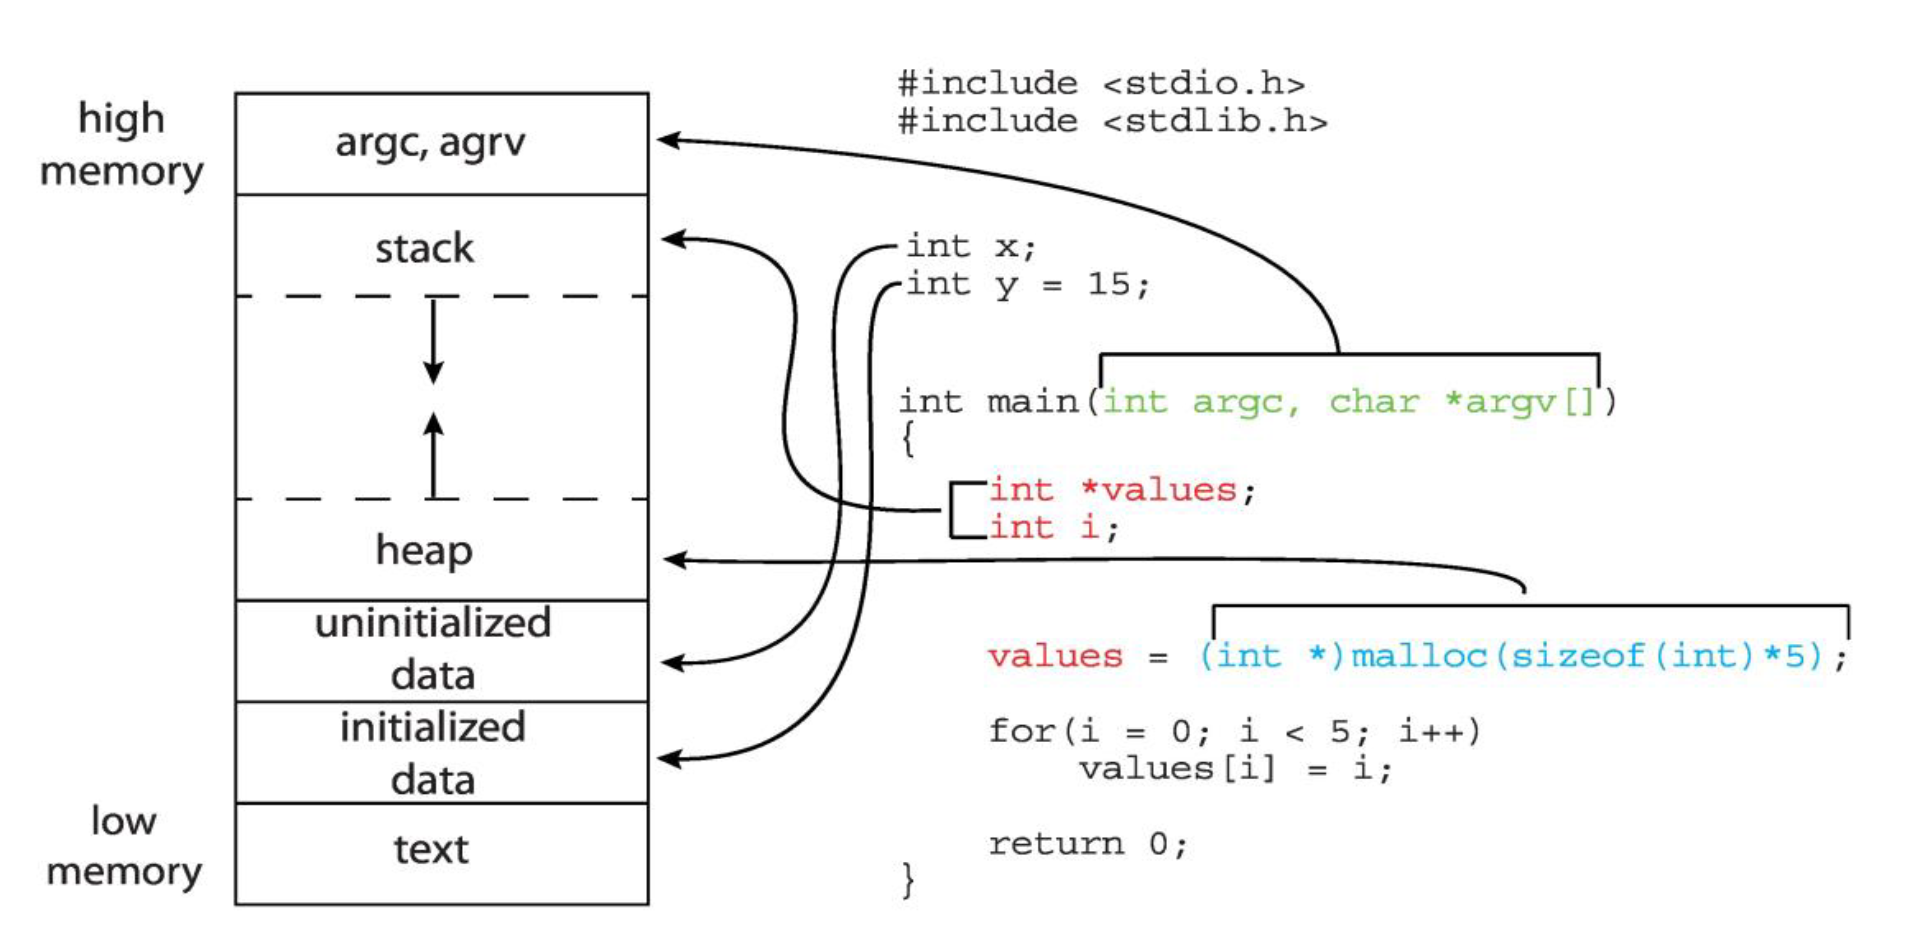
\includegraphics[width=12cm]{unit-8/figures/01.png}
  \caption*{Process memory Layout}
\end{figure}
\subsection{Process Control Block (PCB)}

The information associated with each process is stored as a process control block (PCB), which is also known as a task control block (TCB).
This information includes
\begin{itemize}
  \item process state,
  \item program counter (PC) --- address of next instruction to be executed,
  \item CPU registers,
  \item CPU scheduling information --- priorities and scheduling queue pointers,
  \item memory-management information,
  \item accounting information --- CPU usage, time elapsed and time limits, and
  \item I/O status information --- I/O devices allocated to the processes and list of open files.
\end{itemize}

A process with multiple threads of execution has instructions at multiple addresses executing at once.
This requires multiple program counters.
These additional thread details are stored in the PCB.

\subsection{Process States}

As a process is executed, it changes state.
Possible states for a process are
\begin{itemize}
  \item new --- the process is being created,
  \item ready --- the process is waiting to be assigned to a processor,
  \item running --- the process is executing instructions,
  \item waiting (blocked) --- the process is waiting for an event to occur, and
  \item terminated --- the process has finished execution.
\end{itemize}

When a process is admitted to the system, its state changes from `new' to `ready'.
When it is dispatched to a CPU, its state changes to `running'.
From there, it may time out, in which case its state reverts to `ready', or it may need to wait for an event to occur, in which case its state changes to `blocked'.
Alternatively, it may be released from execution, in which case its state changes to `terminated'.
A process in the `blocked' state moves to the `ready' state once the event it is waiting for occurs.
\begin{figure}[htp]
  \centering
  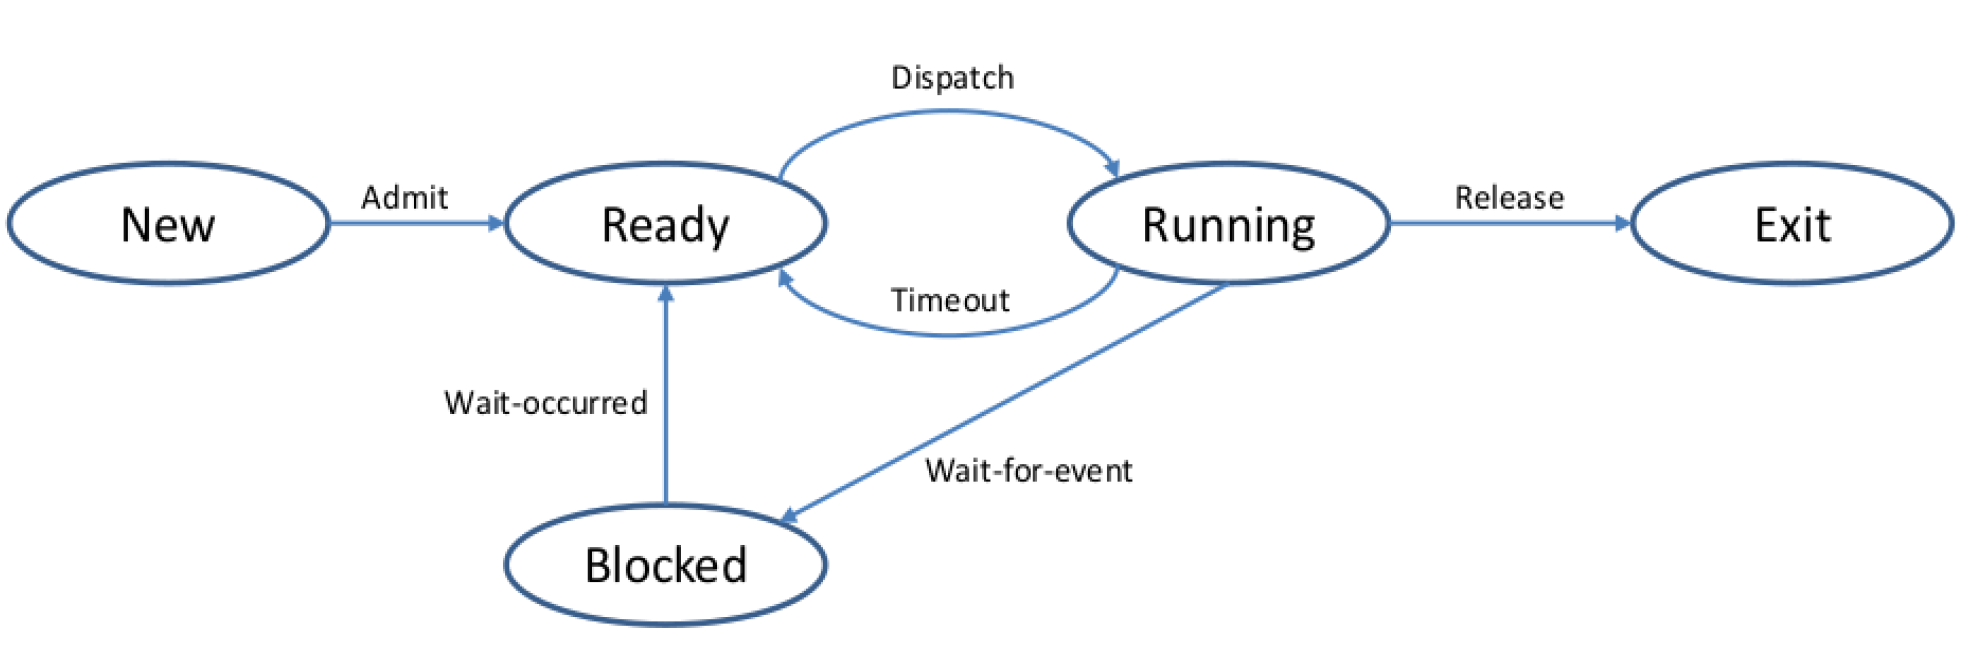
\includegraphics[width=12cm]{unit-8/figures/02.png}
  \caption*{Process memory Layout}
\end{figure}
\subsection{Process Scheduling}

Process scheduling is used to maximise CPU usage and minimise response time by quickly switching processes onto the CPU for time sharing.
A process will `give up' the CPU if it sends an I/O request or after a certain period of time as elapsed.
When a process gives up the CPU, it is added to the ready queue. 
The process scheduler selects available processes in the ready queue for the next execution.

The OS maintains various scheduling queues.
\begin{itemize}
  \item Job queue --- all processes in the entire system
  \item Ready queue --- all processes in main memory ready and waiting to execute
  \item Device queues --- all processes waiting for an I/O device
\end{itemize}

Processes migrate between queues.
Queuing diagrams are used to represent flows of processes and resources.

\subsubsection{Types of Scheduler}

A short-term scheduler (or CPU scheduler) selects which process should be executed next and allocates a CPU\@.
Sometimes this is the only scheduler in a system.
It is invoked frequently and must be fast.

A long-term scheduler (or job scheduler) selects which processes should be brought into the ready queue.
This is invoked infrequently and may be slow.
The long-term scheduler controls the degree of multiprogramming.

\subsubsection{Types of Process}

An I/O-bound process spends more time performing I/O than computations.
It uses many short CPU bursts.
\newline
A CPU-bound process spends more time performing computations.
It uses a few long CPU bursts.
\newline
The long-term scheduler attempts to schedule a good process mix.

\subsubsection{Context Switching}

When the CPU switches to another process, the system saves the state of the old process and loads the saved state of the new process via a context switch.
The context of a process is represented by its PCB.

The time required to perform a context switch is pure overhead; the system does no useful work while switching.
More complex operating systems and process control blocks require more time for a context switch.
The time required is dependent upon hardware support.
Some hardware provides multiple sets of registers per CPU\@.
This allows multiple contexts to be loaded simultaneously.

\begin{figure}[htp]
  \centering
  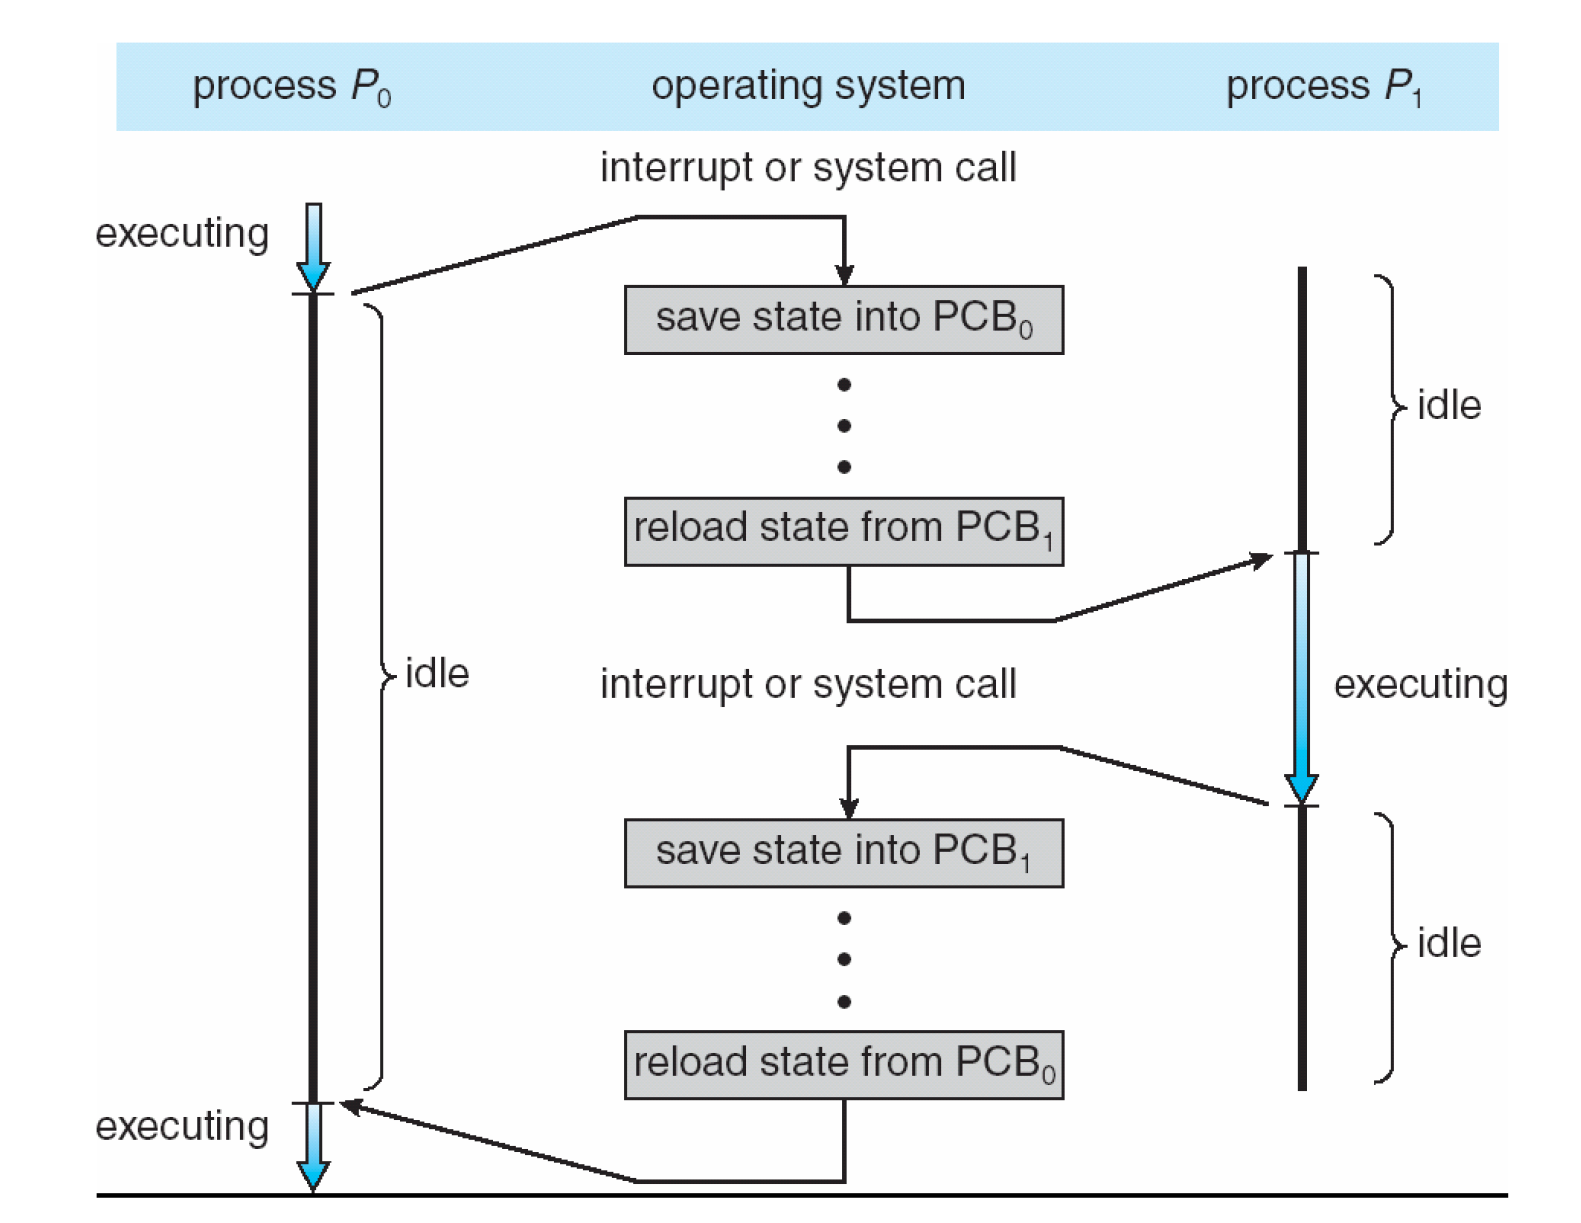
\includegraphics[width=12cm]{unit-8/figures/03.png}
  \caption*{CPU Switch from Process to Process}
\end{figure}
\subsubsection{Dispatch Events}

Context switches (dispatch events) are triggered by clock interrupts.
These occur after a set time interval, typically between \SIlist{3;10}{\milli\second}.
The execution of processes is interrupted and control returns to the OS\@.
The current process is moved to the ready queue.
The frequency of such an interrupt is an important system parameter used to balance the overhead of context switching and the responsiveness of the system.

Context switches are also triggered by I/O interrupts.
When an I/O event occurs and data has been loaded into memory, the current process is interrupted and all blocked processes waiting for the I/O event are moved to the ready queue.
The dispatcher must decide whether to continue execution of the interrupted process.

Memory faults or page faults also trigger context switches.
These occur when an executing process refers to a virtual memory address that has not been allocated a physical memory location (the data requested is still on the disk).
The current process is interrupted and an I/O request for the data is issued.
The current process is moved to the blocked state and execution switches to another process from the ready queue.
When the I/O has completed, the blocked process returns to the ready queue.

\subsubsection{Dispatcher}

A dispatcher is an OS function that allocates processes to the CPU and switches the CPU between processes.
The weakness of a dispatcher with a single device queue is that all processes waiting for an event must be transferred from the device queue to the ready queue when an event occurs.
A dispatcher with multiple queues for different device events moves only the processes waiting for that particular event to the ready queue.

\subsubsection{Virtualisation and Swapping}

A computer system may appear to allow an unlimited number of processes to occur concurrently.
Not all of these processes can fit into physical memory.
It is useful, therefore, to achieve medium-term scheduling and reduce the degree of multiprogramming by removing a process from memory.

Moving a process between memory and storage is known as `swapping'.
This requires two additional process states: `ready-suspended' and `blocked-suspended'.

A process in the `ready-suspended' or `blocked-suspended' state is activated to the `ready' or `blocked' state when it is swapped into memory.
It is suspended when it is swapped out of memory.
A process in the `blocked-suspended' state is moved to the `ready-suspended' state when the event for which it is waiting has occurred.
A process in the `running' state may be suspended.

\subsection{Process Creation}

The system must provide mechanisms for process creation and process termination.

Processes are created at system boot, when an existing process spawns a child process, when the user requests the creation of a process, or when a batch systems executes its next job.
When a parent process creates a child process, a tree of processes is formed.
A process is identified and managed via its process identifier (PID).

When a process is created, it is assigned a unique PID, memory is allocated for its process image, its PCB is initialised, and it is added to the ready queue.

\subsubsection{Parent and Child Processes}

A child process may share all the resources of its parent, a subset of those resources or none of them.
A parent and child process may execute concurrently, or the parent may wait for its children to terminate.

A child process is a duplicate of the address space of its parent.
The child process may load a new program into its address space.

\subsubsection{Process Creation in Unix}

A process creates new processes with the kernel system calls \texttt{fork()} and \texttt{exec()}.
\begin{itemize}
  \item A new slot is allocated in the process table.
  \item A unique PID is assigned to the child process.
  \item The process image of the parent is copied, apart from the shared memory areas.
  \item The child process owns the same open files as the parent.
  \item The child process is added to the ready queue.
\end{itemize}

When \texttt{fork()} is called by the parent process, execution switches to kernel mode and the OS creates a copy of the parent process.
This includes the program code in the text segment of the process image.
Thus, the \texttt{fork()} call is also copied.
The parent process continues execution at the return from the \texttt{fork()} call.
The child process begins execution at the return from the \texttt{fork()} call.

In the parent process, the \texttt{fork()} call returns the PID of the child process.
In the child process, the  \texttt{fork()} call returns zero.
This is used by the remainder of the program to identify whether it is running as a parent or a child.
The program may perform different instructions in either of these cases.

For example, the child process may execute the \texttt{exec()} system call, which takes a program name as a parameter.
This system call replaces the content of the child process image with a process image of the specified program.
\begin{figure}[htp]
  \centering
  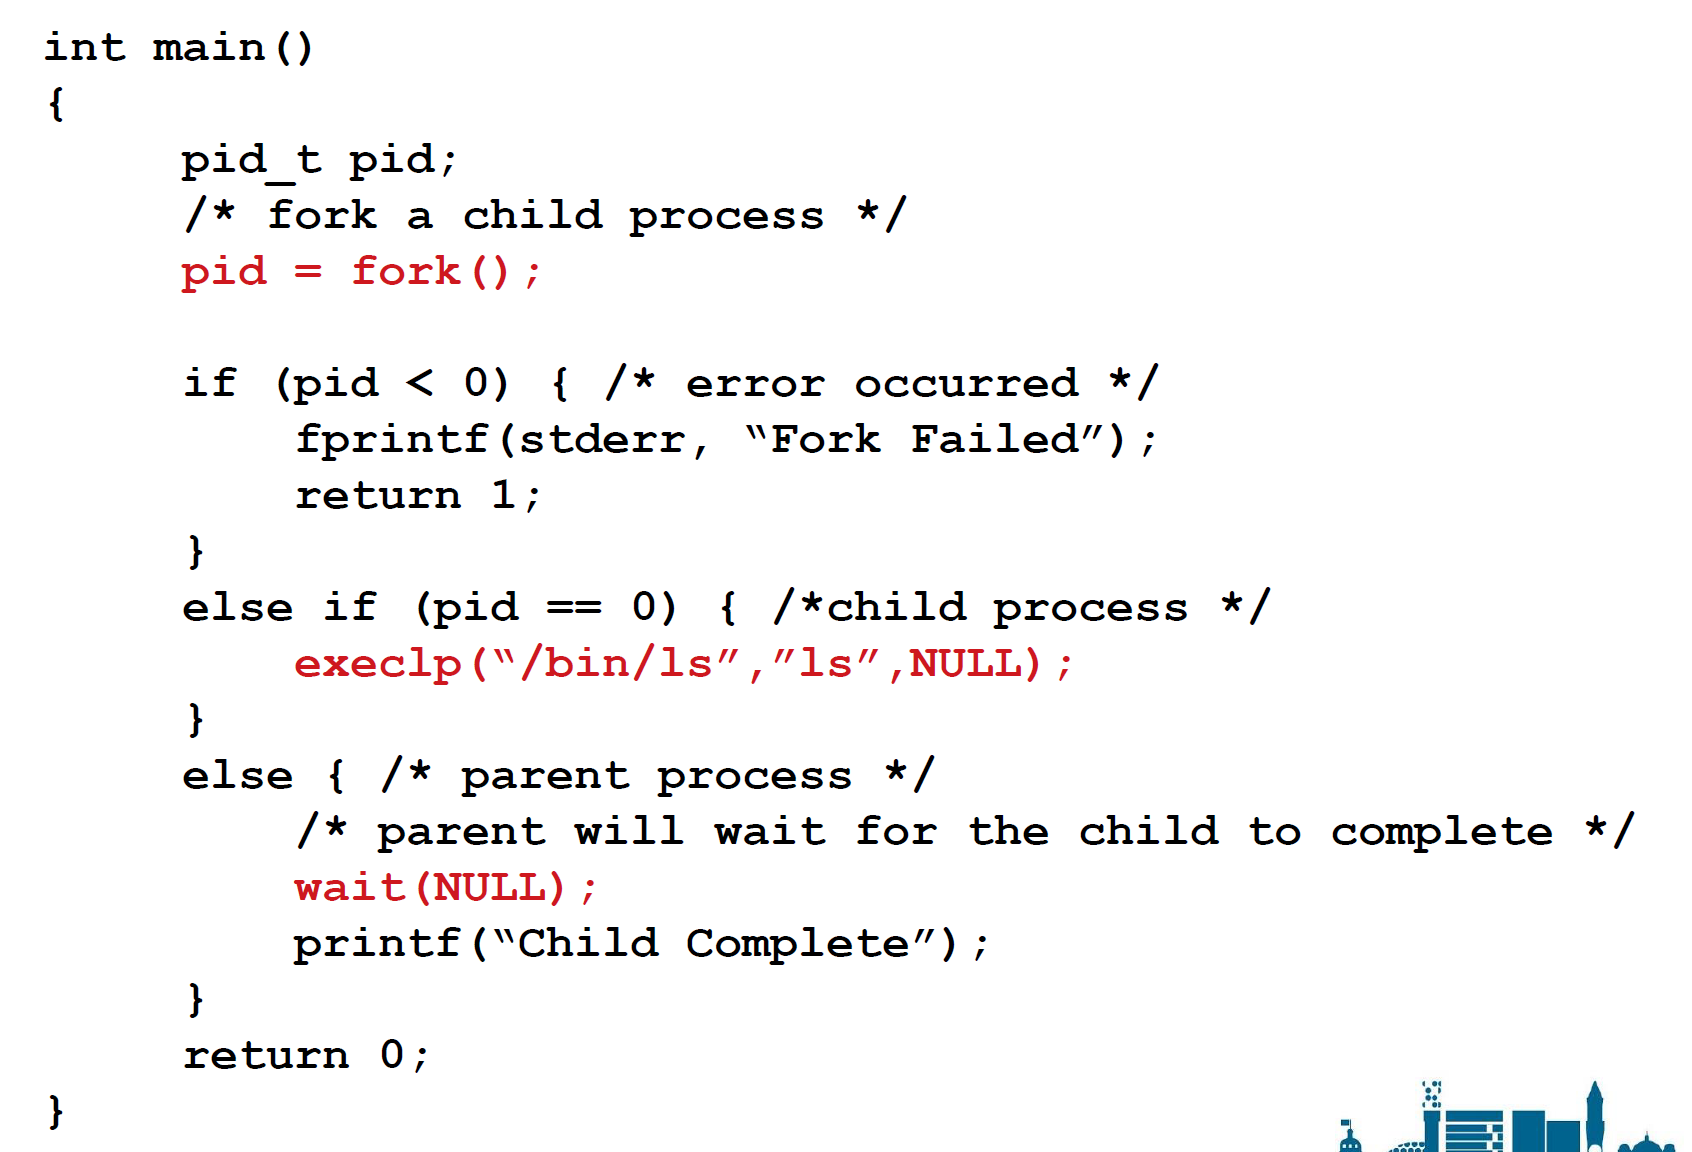
\includegraphics[width=12cm]{unit-8/figures/04.png}
  \caption*{C program to create a separate process in UNIX}
\end{figure}
The \texttt{exec()} system call has a number of variations with different suffixes that describe what parameters are passed to the new process image.
These variations are \texttt{execl()}, \texttt{execle()}, \texttt{execlp()}, \texttt{execv()}, \texttt{execve()} and \texttt{execvp()}.

\begin{itemize}
  \item \texttt{e} --- An array of pointers of environment variables is passed.
  \item \texttt{l} --- Command line arguments are passed individually.
  \item \texttt{p} --- The \texttt{PATH} environment variable is used to find the program to be executed.
  \item \texttt{v} --- Command line arguments are passed as an array of pointers.
\end{itemize}

\subsection{Process Waiting}

A parent may use the system call \texttt{waitpid()} to wait for the termination of a child process.

\subsection{Process Termination}

There are a number of ways in which a process may be terminated.
\begin{itemize}
  \item Normal termination (voluntary) or error termination (voluntary)
  \begin{itemize}
    \item the process reaches regular completion, with or without an error code
  \end{itemize}
  \item Abnormal termination (involuntary)
  \begin{itemize}
    \item OS or user intervenes with kill signal
    \item process attempts to access forbidden memory locations
    \item process times out
    \item process encounters an I/O error
    \item stack overflow
    \item parent process is terminated
  \end{itemize}
\end{itemize}

Some operating systems do not allow a child process to exist if its parent has been terminated.
This is known as `cascading termination'.

A `zombie process' is a process that has terminated but still has an entry in the process table.
This occurs when a child process terminates.
It allows a parent process to read the exit codes of its children.

{\color{gray}
\subsection{Execution of the Operating System}

An OS may be designed so that it executes
\begin{itemize}
  \item separately from processes (non-process kernel),
  \item as part of the user process images (with mode switching), or
  \item as a set of processes (microkernel, with mode and context switching).
\end{itemize}

\subsubsection{Non-Process Kernel OS}

The kernel acts as a monitor for user processes.
All processes are user processes.
There is no concurrent execution of user processes and the kernel; the kernel may execute only during interruptions.

The OS code is placed in a reserved memory region and executes in privileged mode.
It has its own system stack.

\subsubsection{OS Execution within User Processes}

The user address space includes kernel functions.
System functions may be called from within a process by switching to kernel mode.
No context switching is required as the system functions execute within the same process.
The dispatcher executes context switches outside of processes.

\subsubsection{Process-Based OS}

Kernel functions run in kernel mode as separate processes.
The dispatcher handles context switching separately.
This allows concurrency within the kernel, with kernel processes scheduled together with user processes.
This is useful in multiprocessor environments, as kernel functionality may be distributed amongst CPU cores.
}
\subsection{Basic Concepts}

\subsubsection{CPU and I/O Burst Cycle}

Process scheduling is the process of selecting the next process in the ready queue to be executed by the CPU\@.
Scheduling decisions take place when events interrupt the execution of a process.
Such events include 
\begin{itemize}
  \item Clock Interrupts (i.e. process running → ready state)
  \item I/O Interrupts (i.e. process waiting → ready state)
  \item Operating System Calls (read, write, process ready → waiting)
  \item Signals (e.g. Semaphores)
\end{itemize}

Process execution is a cycle of CPU execution and I/O waiting.
Processes on a batch system are CPU-bound, whereas processes on an interactive system are I/O-bound with very short CPU bursts.
When a process is in an I/O burst, the CPU becomes idle and the short-term scheduler must select another process from the ready queue.
The ready queue is not necessarily a FIFO queue; it may be a priority queue, tree or unordered linked list.

\subsubsection{Dispatcher}

The dispatcher is the module that gives control of the CPU to the process selected by the short-term scheduler.
This involves switching context, switching to user mode and jumping to the correct location stored in the PCB of the process in order to resume execution.
The dispatcher must be as fast as possible since it is invoked at every process switch.
The time taken by the dispatcher to stop one process and start another is known as `dispatch latency'.

\subsubsection{Levels of Scheduling}

The long-term scheduler is responsible for admitting new processes to the ready queue.
The short-term scheduler is responsible for selecting the next process to be given control of the CPU\@.
The mid-term scheduler is responsible for moving processes between suspended and non-suspended states.

A non-preemptive scheduler allows an executing process to continue execution until it terminates, releases the CPU voluntarily (cooperative scheduling) or is blocked due to an event such as an I/O interrupt.
A preemptive scheduler may stop an executing process due to a clock interrupt (time slice expired) or when a process with a higher priority becomes ready.

\subsection{Scheduling Criteria}

Scheduling algorithms are designed to maximise or minimise different parameters.
OS parameters to be maximised include

Many criteria suggested, including
\begin{itemize}
\item CPU Utilization - keep that CPU as busy as possible. 0-100\%, but realistically, 40-90%
\item Throughput - Number of processes that complete their execution per time unit
\item Turnaround time - Total amount of time to execute one process to its completion.
\item Waiting time - Total amount of time a process has been waiting in the Ready queue
\item Response time - The time it takes from when a request was submitted until the first response is produced by the operating system (latency).
\end{itemize}
Others include meeting deadlines, predictability, fairness, balance and enforcing priorities


\subsection{Scheduling Algorithms}

\subsubsection{First Come First Serve (FCFS)}

First come first serve (FCFS) is the simplest scheduling algorithm.
Processes are given control of the CPU in the order that they request it.
This is implemented with a FIFO ready queue.
When a process enters the ready queue, its PCB is pushed to the tail.
When the CPU becomes free, it is allocated to the process whose PCB is popped from the head of the queue.

Using this algorithm, the average process waiting time can vary greatly.
If a long process arrives before a short process, the waiting time for the second process will be long.
If the short process arrives first, the second process will have a short waiting time.

Suppose the processes arrive in the order: P1 , P2 , P3. Gantt Chart as follows:
\renewcommand{\arraystretch}{2} % row height

\begin{center}
\begin{tabular}{|>{\centering\arraybackslash}m{4cm}|>{\centering\arraybackslash}m{4cm}|}
\hline
\textbf{Process} & \textbf{Burst Time} \\
\hline
P\textsubscript{1} & 24 \\
\hline
P\textsubscript{2} & 3 \\
\hline
P\textsubscript{3} & 3 \\
\hline
\end{tabular}
\end{center}

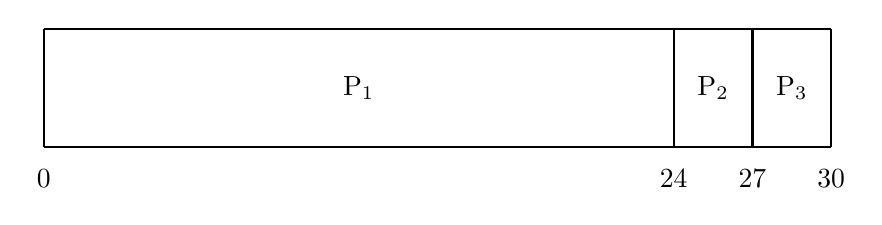
\begin{tikzpicture}
  % Draw the timeline
  \draw[thick] (0,0) -- (10,0); % Total length
  \draw[thick] (0,0) -- (0,1.5);   % Left side
  \draw[thick] (8,0) -- (8,1.5);   % Divider for P1 end
  \draw[thick] (9,0) -- (9,1.5);   % Divider for P2 end
  \draw[thick] (10,0) -- (10,1.5); % Right side
  \draw[thick] (0,1.5) -- (10,1.5);% Top side

  % Labels for processes
  \node at (4,0.75) {P\textsubscript{1}};
  \node at (8.5,0.75) {P\textsubscript{2}};
  \node at (9.5,0.75) {P\textsubscript{3}};

  % Time labels
  \node at (0,-0.4) {0};
  \node at (8,-0.4) {24};
  \node at (9,-0.4) {27};
  \node at (10,-0.4) {30};
\end{tikzpicture}

Waiting time for P1 = 0; P2 = 24; P3 = 27
Average waiting time: (0 + 24 + 27)/3 = 17ms

\subsubsection{Shortest Job First (SJF)}

Using the shortest job first (SJF) scheduling algorithm, each process is associated with an estimate of the length of its next CPU bust.
When the CPU becomes available, it is assigned to the process that has the shortest estimated next CPU burst.
If two processes are estimated to have next CPU bursts of the same length, FCFS is used to choose between them.
A more accurate name for this algorithm would be `shortest next CPU burst first'.

The SJF scheduling algorithm can be proven to be optimal.
It gives the minimum average waiting time for a given set of processes.
This works because scheduling a short process before a long process decreases the waiting time of the short process more than it increases the waiting time of the long process.
Thus, the average waiting time decreases.

However, the algorithm is difficult to implement since there is no way to know the exact length of the next CPU burst.
Instead, the length of the next CPU burst of a process is estimated by an exponential average of the measured lengths of its previous CPU bursts.
The predicted length \( \tau_{n + 1} \) of the next (\( \left( n + 1 \right) \)th) CPU burst is given by the following iterative formula in terms of the measured length \( t_n \) of the previous (\( n \)th) CPU burst and a weighting factor \( \alpha \).

\begin{equation*}
  \tau_{n + 1} = \alpha t_n + \left( 1 - \alpha \right) \tau_n
\end{equation*}

Commonly, the weighting factor \( \alpha \) is set to \num{0.5}.
Thus, if the predicted and actual lengths of the \( n \)th CPU burst are \SIlist{10;6}{\milli\second}, respectively, the predicted length of the \( \left( n + 1 \right) \)th CPU burst would be \SI{8}{\milli\second}.

\subsubsection{Shortest Remaining Time First (SRTF)}

SJF can be either preemptive or non-preemptive.
If the length of the next CPU burst of a newly submitted process is shorter than the remaining CPU burst of the currently executing process, the preemptive SJF would switch the two processes to minimise the average waiting time, whereas the non-preemptive SJF would allow the current process to finish its CPU burst.

The preemptive SJF scheduling algorithm is known as the `shortest remaining time first' (SRTF) scheduling algorithm.

\subsubsection{Priority Scheduling}

The SJF scheduling algorithm is a special case of the general priority scheduling algorithm.
A priority is associated with each process and the CPU is allocated to the process with the highest priority.
Priorities are indicated by a fixed range of numbers.
Lower numbers are used for higher priorities.
Processes with equal priorities are scheduled using FCFS.

Priorities can be defined by internal criteria, such as time limits, memory requirements and number of open files, or external criteria, such as process importance, funds paid for computation or political factors.

Preemptive priority scheduling will switch processes if a newly submitted process has a higher priority than the current process.
Non-preemptive priority scheduling would simply place that process at the head of the priority queue.

Priority scheduling can result in the indefinite blocking or starvation of low-priority processes if the system receives a steady stream of processes with higher priority.
These processes may eventually run after a very long waiting time, or may be lost if the system crashes before that point.
\newline
This can be solved by increasing priority with age.

\subsubsection{Round-Robin (RR)}

The round-robin (RR) scheduling algorithm is designed especially for time-sharing systems.
It is similar to FCFS, but uses preemption to enable the switching of processes.
A circular ready queue and small `time quantum' or `time slice' are used.
The CPU is allocated to each process in the queue for a time interval of up to one time quantum.
The ready queue is treated as a FIFO queue.

The scheduler sets a timer to interrupt the CPU after one time quantum and dispatches the first process in the ready queue.
If the process has a CPU burst length of less than one time quantum, the process will release the CPU voluntarily.
Otherwise, the process is interrupted after one time quantum, resulting in a context switch to the second process.
The first process is pushed to the tail of the ready queue.

If there are \( n \) processes in the ready queue and the time quantum is \( q \), each process is given \( \frac{1}{n} \) of the CPU time in bursts of at most \( q \).
Each process must wait no longer than \( \left( n - 1 \right) q \) until its next CPU burst.
For example, in a queue of five processes with a time quantum of \SI{20}{\milli\second}, each process is given up to \SI{20}{\milli\second} of CPU time every \SI{100}{\milli\second} or less, resulting in a waiting time of no more than \SI{80}{\milli\second} between CPU bursts.

The performance of the RR scheduling algorithm depends heavily on the size of the time quantum.
If the time quantum is longer than the process length, the algorithm would be no different from FCFS\@.
If the time quantum is too short, there would be a large number of expensive context switches.
Ideally, the time quantum should be much larger than the context switch time.
If the context switch time is \( n \)\si{\percent} of the time quantum, approximately \( n \)\si{\percent} of CPU time would be devoted to context switching.
Modern systems typically have time quanta between \SIlist{10;100}{\milli\second} and context switches of less than \SI{10}{\micro\second}.


\subsubsection{Appandix}
Introduction to Operating Systems:
Definition and role of an OS in managing hardware and software resources.
Components of a computer system (Hardware, OS, Application, Users).
Operating System Services \& Evolution:
Key functions like process management, memory management, I/O operations, file systems, and security.
Transition from Uniprogramming to Multiprogramming, and Time-Sharing systems.

Computer Architecture \& OS Structures
Bootstrapping process, Main Memory and I/O structure.
Overview of how I/O devices interact with the system.
Types of I/O mechanisms and their role in performance.
Process Management \& Scheduling
The concept of processes, their lifecycle (process states), and operations on processes.
Scheduling criteria: efficiency, fairness, response time, throughput, etc.
Common Scheduling Algorithms including FCFS, SJF, SRTF, Priority \& Round-Robin.